\chapter{\textit{Compressive Sensing}}

\textit{Compressive Sensing} (CS), também conhecido como \textit{Compressive Sampling} ou \textit{Compressed Sensing},  estuda formas de reconstruir um vetor a partir de poucas amostras. De agora em diante, iremos assumir que as amostras $(y_i)_{i = 1}^m$, representadas pelo vetor $y \in \mathbb{R}^m$ de um sinal $x \in \mathbb{R}^n$ são obtidas a partir de uma transformação linear $y = Ax$, onde $A$ é uma matriz $m \times n$, com $m < n$.

{\bf Observação:} Durante o texto, sempre que referirmos a um vetor como uma imagem, assumimos que o vetor é calculado ao empilhar todas as linhas da imagem em escala de cinza.

Como \newc{$m < n$}, a equação não possui uma única solução $x$, se possuir. Podemos escolher o vetor $x$ que minimiza $\Vert Ax - y \Vert_2^2$, pelo método de mínimos quadrados. $x$ pode ser calculado como $x = A^{\dagger} y$, onde $A^{\dagger}$ denota a pseudo-inversa de $A$. Porém as imagens recuperadas dessa forma não são parecidas com a imagem original.

A Figura $\ref{fig:mmq}$ mostra uma imagem recuperada pelo método de mínimos quadrados para uma matriz $A$ $m \times n$, onde $m = 80 \% \cdot n$ (compressão de $20\%$) e as entradas de $A$ são independentes e seguem a distribuição normal com média $0$ e variância $1$.

%Nesse caso dizemos que as entradas de $A$ são iid $\mathcal{N}(0,1)$ onde, com iid queremos dizer que os elementos foram calculados de forma independente e que todos a mesma distribuição de probabilidade. $\mathcal{N}(0,1)$ denota a distribuição normal com média $0$ e variância $1$).

\afterpage{
\begin{figure}
\centering
	\begin{subfigure}[b]{0.4\textwidth}
        \centering
        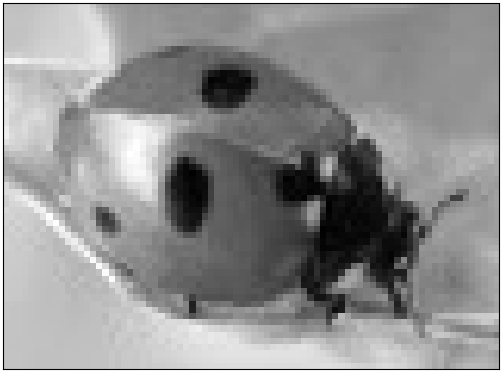
\includegraphics[scale=.35]{imagens/homotopy/joaninha.png}
        \caption{imagem original}
%	    \label{fig:homotopy/original.png}
    \end{subfigure}
    ~
    \begin{subfigure}[b]{0.4\textwidth}
        \centering
        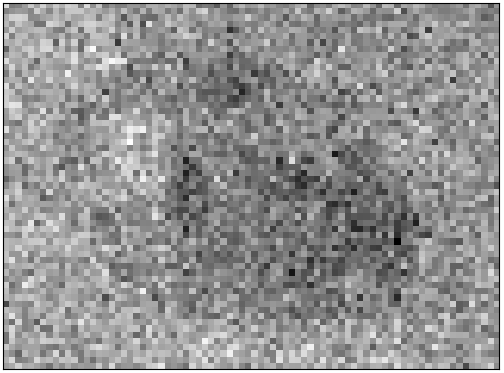
\includegraphics[scale=.35]{imagens/homotopy/joaninhaMMQ_20porcento.png}
        \caption{compressão de $20\%$}
%	    \label{fig:homotopy/80porcentoMMQ.png}
    \end{subfigure}
    \caption{Recuperando imagem usando o método de mínimos quadrados para $y = Ax$, onde o vetor $x$ representa a imagem original e $A$ é uma matriz $m \times n$ com $m = 80 \% \cdot n$\newc{ (compressão de $20\%$)} cujas entradas seguem a distribuição normal de média $0$ e variância $1$ e são calculadas independentemente. Adaptado de \small{\protect\url{https://commons.wikimedia.org/wiki/File:5-stip_LHB_09.jpg}}}
    \label{fig:mmq} %label deve ficar após caption
\end{figure}
%\footnotetext{\url{https://commons.wikimedia.org/wiki/File:5-stip_LHB_09.jpg}}
}
Sabemos que geralmente imagens são esparsas no espectro da frequência. Uma imagem pode ser decomposta como uma combinação linear de senoidais e, na prática, os coeficientes correspondentes às frequências mais altas são muito próximos de zero. Na Figura $\ref{fig:coeficientes_altos}$ a imagem é reconstruída apenas com as frequências cujos coeficientes estão entre os $60\%$ maior valor absoluto (compressão de $40\%$). Note que as imagens {\bf (a)} e {\bf (b)} são bastante parecidas, indicando que a imagem é esparsa, ou aproximadamente esparsa (com muitos coeficientes próximos de zero) no espectro da frequência. 

\afterpage{
\begin{figure}
\begin{center}
	\begin{subfigure}[b]{1\textwidth}
        \centering
        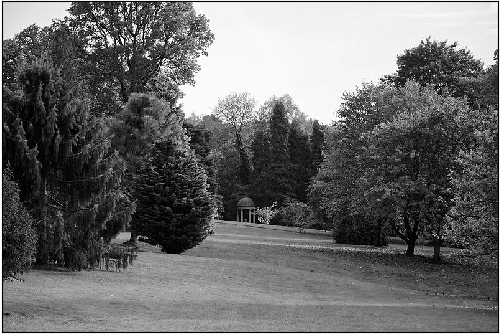
\includegraphics[scale=.7]{imagens/Beale_Arboretum_gray.png}
        \caption{imagem original}
%	    \label{fig:homotopy/originals.png}
    \end{subfigure}
    \\
    \begin{subfigure}[b]{1\textwidth}
        \centering
        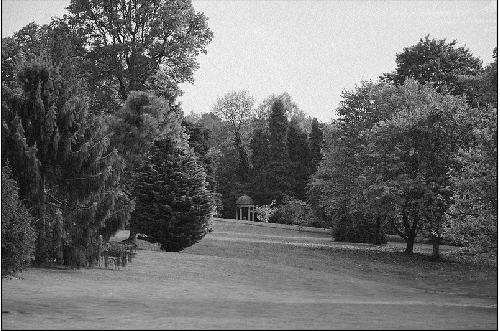
\includegraphics[scale=.7]{imagens/Beale_Arboretum_60porc_freq_maiores.png}
        \caption{compressão de $40\%$}
%	    \label{fig:homotopy/80porcentoMMQ.png}
    \end{subfigure}
    \caption[]{A imagem em {\bf (b)} é calculada ao descartar $40\%$ das senoidais que compõem a imagem cujos coeficientes têm menor módulo. Adaptado de \\ \small{\protect\url{https://commons.wikimedia.org/wiki/File:Along_The_Main_Ride_-_Beale_Arboretum}  \\\protect\url{_-_West_Lodge_Park_-_Hadley_Wood_-_Enfield_London_2.jpg}}}
     \label{fig:coeficientes_altos}
\end{center}
\end{figure}
%\footnotetext{ \url{https://commons.wikimedia.org/wiki/File:Along_The_Main_Ride_-_Beale_Arboretum_} \\ \url{-_West_Lodge_Park_-_Hadley_Wood_-_Enfield_London_2.jpg} }
}

A ideia é então escolher, entre todas as soluções possíveis, o vetor $x$ com o maior número de coeficientes nulos. Para entender melhor o problema, as seguintes definições, retiradas de \cite{ddek}, serão enunciadas:

\textbf{Def:} Seja $x \in \mathbb{R}^n$. $x$ é $k$-esparso se possui, no mínimo, $k$ coeficientes nulos.

\textbf{Def:} Dado $x \in \mathbb{R}^n$, a `norma' $0$ de $x$ é definida como
$\Vert x \Vert_{0} = \# \lbrace i : \vert x_i \vert > 0 \rbrace$, ou seja, a quantidade de elementos não nulos de $x$. \footnote{Denotaremos a quantidade de elementos em um conjunto $I$ arbitrário como $\# I$.}

Observe que a `norma' 0 não é uma norma, pois, se $x = (1, 0)$, $\Vert 2x \Vert = 1 \neq 2 \Vert x \Vert$. Porém, $\Vert \cdot \Vert_0$ satisfaz as propriedades demonstradas na Proposicao $\ref{prp:norma_0}$, retirada de \cite{ddek}.

\begin{proposicao}
Fixados $x, y \in \mathbb{R}^n, \lambda \in \mathbb{R}$, a `norma' $0$ satisfaz as seguintes propriedades:
\begin{enumerate}[(i)]
\item $\Vert x \Vert_0 \geq 0$
\item $\Vert x \Vert_0 = 0 \Leftrightarrow x = 0$
\item Se $\lambda \neq 0, \Vert \lambda x \Vert_0 \neq \vert \lambda \vert \Vert x \Vert_0$
\item $\Vert x + y \Vert_0 \leq \Vert x \Vert_0 + \Vert y \Vert_0$
\item A norma $0$ não é uma norma.
\end{enumerate}
\label{prp:norma_0}
\end{proposicao}
\begin{proof}

Fixados $x, y \in \mathbb{R}^n, \lambda \in \mathbb{R}$

\begin{enumerate}[(i)]
\item $\Vert x \Vert_0 = \# \lbrace i \in \lbrace 1, \hdots, n \rbrace: \vert x_i \vert > 0 \rbrace \geq 0$
\item \begin{subequations}
\begin{align*}
\Vert x \Vert_0 = 0 &
\Rightarrow \# \lbrace i \in \lbrace 1, \hdots, n \rbrace: \vert x_i \vert > 0 \rbrace = 0 \\
& \Rightarrow \forall i \in \lbrace 1, \hdots, n \rbrace, \vert x_i \vert = 0 \\
& \Rightarrow x = 0
\end{align*}
\end{subequations}

\item Se $\lambda \neq 0$,
\begin{subequations}
\begin{align*}
\Vert \lambda x \Vert_0 & = \# \lbrace i \in \lbrace 1, \hdots, n \rbrace: \vert \lambda x_i \vert > 0 \rbrace \\
& = \# \lbrace i \in \lbrace 1, \hdots, n \rbrace: \vert x_i \vert > 0 \rbrace\\
& = \Vert x \Vert_0
\end{align*}
\end{subequations}

Então, para $x \neq 0$ e $\lambda \notin \lbrace 0, 1 \rbrace$, temos que
\begin{subequations}
\begin{align*}
\Vert \lambda x \Vert_0 & = \Vert x \Vert_0 \text{, pelo item $(i)$} \\
& \neq \vert \lambda \vert \Vert x \Vert_0
\end{align*}
\end{subequations}
\item
\begin{subequations}
\begin{align*}
\Vert x \Vert_0 + \Vert y \Vert_0 & = \# \lbrace i : \vert x_i \vert > 0 \rbrace
									+ \# \lbrace i : \vert y_i \vert > 0 \rbrace \\
& \geq \#(\lbrace i : \vert x_i \vert > 0 \rbrace \cup \lbrace i : \vert y_i \vert > 0 \rbrace) \\
& = \# \lbrace i : \vert x_i \vert > 0 \textit{ ou } \vert y_i \vert > 0 \rbrace \\
& = \# \lbrace i : \vert x_i \vert + \vert y_i \vert > 0 \rbrace \\
& \geq  \# \lbrace i : \vert x_i + y_i \vert > 0\rbrace \\
& = \Vert x + y \Vert_0
\end{align*}
\end{subequations}

\item Sejam $\lambda = 2, x = e_1$, então

$$ \Vert \lambda x \Vert_0 = \Vert x \Vert_0 = 1 \neq \vert \lambda \vert \Vert x \Vert_0 $$

Então a norma $0$ não é uma norma.
\end{enumerate}
\end{proof}

O problema que resolveremos para encontrar o vetor $x$ mais esparso amostrado como $x = Ay$ será formulado do seguinte modo:

\begin{equation}
\tag{$P_0$}
\min_{x \in \mathbb{R}^n} \Vert x \Vert_{0} \textit{ sujeito a } Ax = y
\label{eqn:P0}
\end{equation}

No entanto, $\eqref{eqn:P0}$ é NP-difícil \cite{fourau} (NP, ou tempo polinomial não determinístico, denota a classe de problemas que podem ser verificados em tempo polinomial. Ainda não sabemos se esses problemas podem ser resolvidos em tempo polinomial). Então tentamos resolver o seguinte problema:

\begin{equation}
\tag{$P_1$}
\min_{x \in \mathbb{R}^n} \Vert x \Vert_{1} \textit{ sujeito a } Ax = y
\label{eqn:P1}
\end{equation}

A Figura $\ref{fig:normas}$ nos ajuda a entender a semelhança entre $\eqref{eqn:P0}$ e $\eqref{eqn:P1}$. A figura mostra o problema de minimização de $\Vert x \Vert_p$ sujeito a $Ax = y$ para $x \in \mathbb{R}^2$ e $y \in \mathbb{R}$. O ponto $x$ minimiza a norma em um único ponto se a fronteira de uma bola fechada centrada em $0$ toca a reta $Ax = y$ apenas em $x$. Neste caso, as soluções calculadas para $p = 1$ e $p = 1/2$ são esparsas. Note que $\Vert \cdot \Vert_{\frac{1}{2}}$ não é norma.

\begin{figure}
\centering
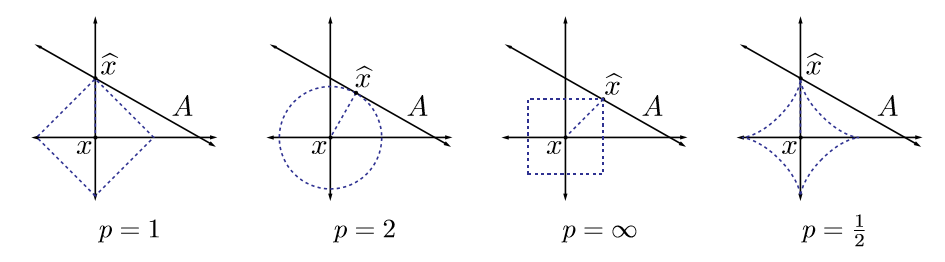
\includegraphics[scale=.6]{imagens/normas.png}
\caption{Pontos na reta $Ax = y$ que minimizam a norma $\Vert \cdot \Vert_p$ para diferentes valores de $p$. As soluções encontradas para $p = 1$ e $p = 1/2$ são esparsas. Note que $\Vert \cdot \Vert_{\frac{1}{2}}$ não é norma. Reproduzido de \cite{ddek}.}
\label{fig:normas}
\end{figure}

CS tem como objetivo estudar condições para garantir a equivalência entre os dois problemas, e condições para a unicidade de soluções de $\eqref{eqn:P0}$ e $\eqref{eqn:P1}$. Descrevemos estas condições nas seções 3.1, 3.2 e 3.43 Todos resultados mostrados nessas seções podem ser encontrados em \cite{ddek}, exceto quando indicados explicitamente.

\section{Unicidade de $\eqref{eqn:P0}$}
Se a matriz $A$ fosse $n \times n$ de posto máximo, a unicidade estaria garantida. Como $m < n$, definimos o conceito de \textit{spark}, que verbalmente é uma fusão dos conceitos `esparso' e `posto' (\textit{rank}) \cite{kutyniok}.

\begin{definicao}
Seja $A$ uma matriz $m \times n$. O \textit{spark} de $A$, denotado por $\textit{spark}(A)$, é o menor número de colunas linearmente dependentes de $A$ (ou de forma equivalente, $spark(A)$ é o menor número de colunas LD de $A$)\footnote{Dizemos que um conjunto de colunas é LD se elas forem linearmente dependentes. Diremos que uma matriz $A$ é LD se suas colunas forem LD}.
\end{definicao}

O Teorema a seguir nos indica uma condição que $A$ deve satisfazer para garantir a unicidade de $\eqref{eqn:P0}$

\begin{teorema}
\label{thm:unicidade_P0}
Seja $A$ uma matriz $m \times n$. São equivalentes:

\begin{enumerate}[(i)]
\item $\textit{spark}(A)> 2k$

\item Para todo $y \in \mathbb{R}^m$, existe no máximo um $x \in \Sigma_k$ tal que $y = Ax$.
\end{enumerate}
\end{teorema}

Portanto, é desejável que $\textit{spark}(A)$ seja alto pois, nesse caso, seria possível recuperar vetores $x$ não tão esparsos.

Antes de demonstrar o teorema, enunciaremos uma definição e demonstraremos um lema.

\begin{definicao}
Dado $k \in \lbrace 1, \hdots , n \rbrace$,
$ \Sigma_k = \lbrace x : \Vert x \Vert_{0} \leq k \rbrace
           = \lbrace x : x $ é $k$-esparso$ \rbrace$
\end{definicao}

\begin{lema}
Dados $u, v \in \Sigma_k, u - v \in \Sigma_{2k}$
\end{lema}
\label{lem:sigma2k}
\begin{proof}
Sejam $u, v \in \Sigma_k$. Então
\begin{subequations}
\begin{align*}
\Vert u - v \Vert_0 & \leq \Vert u \Vert_0 + \Vert -v \Vert_0 \\
& = \Vert u \Vert_0 + \Vert v \Vert_0 \\
& \leq k + k = 2k \\
& \Rightarrow u - v \in \Sigma_{2k}
\end{align*}
\end{subequations}
\end{proof}

Agora iremos demonstrar o Teorema \ref{thm:unicidade_P0}.
\begin{proof}
Seja $A$ uma matriz $m \times n$. Denote cada coluna $j$ de $A$ por $a_j$.
\begin{itemize}
\item $\neg$(i) $\Rightarrow$ $\neg$(ii)

Suponha que $\textit{spark}(A) \leq 2k$. Então existe um conjunto $J \subset \lbrace 1, \hdots, n \rbrace$  tal que $\#J = 2k$ e existe uma bijeção $\mu$ entre $\lbrace 1, \hdots, 2k \rbrace$ e $J$ tais que

$$ \lbrace a_{\mu(j)} : j \in \lbrace 1, \hdots, 2k \rbrace \rbrace \text{ é LD }$$

Então existe $c \in R^{2k}, c \neq 0$ tal que

$$ \sum_{j = 1}^{2k} c_j a_{\mu(j)} = 0$$

Defina $u, v \in \mathbb{R}^n$ tais que, para $j \in \lbrace 1, \hdots, n \rbrace$

\begin{subequations}
\begin{align*}
u_j = 
\begin{cases}
c_{\mu^{-1}(j)} & \text{ se } j \in \mu^{-1}(\lbrace 1, \hdots, k \rbrace) \\
0, & \text{caso contrário}
\end{cases}
\end{align*}
\end{subequations}

\begin{subequations}
\begin{align*}
v_j = \begin{cases}
 -c_{\mu^{-1}(j)} & \text{ se } j \in \mu^{-1}(\lbrace k+1, \hdots, 2k \rbrace)\\
  0 &\text{ caso contrário}
\end{cases}
\end{align*}
\end{subequations}


Se $j \in \mu^{-1}(\lbrace 1, \hdots, 2k \rbrace), u_j - v_j = c_j$. Então $u \neq v$\\
Então $\Vert u \Vert_0, \Vert v \Vert_0 \leq k \Rightarrow u, v \in \Sigma_k$.

Então
\begin{subequations}
\begin{align*}
\sum_{j = 1}^{2k} c_j a_{\mu(j)} &= \sum_{j = 1}^{k} c_j a_{\mu(j)} + \sum_{j = k+1}^{2k} c_j a_{\mu(j)}\\
& = \sum_{j = 1}^{k} u_{\mu(j)} a_{\mu(j)} - \sum_{j = k+1}^{2k} v_{\mu(j)} a_{\mu(j)} \\
& = Au - Av = 0 \\
 \Rightarrow Au = Av
\end{align*}
\end{subequations}

Então, definindo $y = Au$, existem $u, v \in \mathbb{R}^n$ distintos tais que $Au = Av$.
\item $\neg$(ii) $\Rightarrow$ $\neg$(i)

Suponha que existam $y \in \mathbb{R}^m$, $z, w \in \Sigma_k$ distintos tais que $y = Az = Aw$.

Seja $x = z - w$. Então $Ax = 0$ e, pelo Lema $\ref{lem:sigma2k}$, $x \in \Sigma_{2k}$. Além disso, $x \neq 0$.

Defina $K = \lbrace i \in \lbrace 1, \hdots, n \rbrace: \vert x_i \vert > 0 \rbrace$ e $\mu$ uma bijeção entre $\lbrace 1, \hdots, \Vert x \Vert_0 \rbrace$ e $K$. Então

$$ Ax = \sum_{j = 1}^{\Vert x \Vert_0} a_{\mu(j)} x_{\mu(j)} = 0$$

Como $x \neq 0$, existe algum $j \in \lbrace 1, \hdots, \Vert x \Vert_0 \rbrace$ tal que $x_{\mu(j)} \neq 0$. Logo, $A$ possui $\Vert x \Vert_0$ colunas linearmente dependentes. Portanto, $\textit{spark}(A) \leq \Vert x \Vert_0 \leq 2k$.
\end{itemize}
\end{proof}
\section{Unicidade de $\eqref{eqn:P1}$}

Ao encontrar a solução única de $\eqref{eqn:P0}$, encontramos o vetor desejado. No entanto, $\eqref{eqn:P0}$ é NP-difícil. Uma alternativa seria resolver o problema $\eqref{eqn:P1}$.

Precisamos então estudar a unicidade de soluções para $\eqref{eqn:P1}$ e condições para a equivalência entre $\eqref{eqn:P0}$ e $\eqref{eqn:P1}$, ou seja, condições em que um vetor $x$ é solução única de ambos $\eqref{eqn:P0}$ e $\eqref{eqn:P1}$.

Definimos o conceito de \textit{Null space property} para estudar a unicidade de $\eqref{eqn:P1}$.

\begin{definicao} Seja $\Lambda \subset \lbrace 1, 2, \hdots, n \rbrace$. Defina $\Lambda^{\mathsf{c}} = \subset \lbrace 1, 2, \hdots, n \rbrace \setminus \Lambda$. Dado $x \in \mathbb{R}^n, x_{\Lambda} \in \mathbb{R}^n$, onde, para i $\in [n] = \{1, \hdots, n\}$

$$(x_{\Lambda})_i = 
\begin{cases}
x_i, &\mbox{se } i \in \Lambda \\
0,   &\mbox{caso contrário}
\end{cases}$$

\end{definicao}

\begin{definicao} Uma matriz A de tamanho $m \times n$ satisfaz a \textit{null space property} (NSP) relativa ao conjunto $\Lambda \subset [n]$ se para todo $h \in \ker(A) \setminus \lbrace 0 \rbrace$
%de ordem $k$ se existir uma constante $C > 0$ tal que

%para todo $h \in \ker(A), \Lambda \subset \lbrace 1, \hdots, n \rbrace \text{ tal que } \vert \Lambda \vert \leq k,$
%$$ \Vert h_{\Lambda} \Vert_2 \leq \frac{C \Vert h_{\Lambda^{\mathsf{c}}} \Vert_1}{\sqrt{k}} $$

%Estou usando a definicao do livro
$$ \Vert h_{\Lambda} \Vert_1 <  \Vert h_{\Lambda^{\mathsf{c}}} \Vert_1$$
\end{definicao}

\begin{definicao}
Dizemos que uma matriz de tamanho $m \times n$ satisfaz a \textit{null space property} (NSP) de ordem $k$ se ela satisfaz a NSP para todo $\Lambda \subset [n]$ com $\# \Lambda \leq k$.
\end{definicao}

\begin{lema}
Seja $\Lambda \in [n]$. Dado $x \in \mathbb{R}^n,$

$$ \Vert x \Vert_1 = \Vert x_{\Lambda} \Vert_1 + \Vert x_{\Lambda^{\mathsf{c}}} \Vert_1 $$
\end{lema}
\begin{proof} %Follow your nose.
$$
\Vert x \Vert_1 = \sum_{j = 1}^n \vert x_j \vert
= \sum_{j \in \Lambda}^n \vert x_j \vert + \sum_{j \in \Lambda^{\mathsf{c}}}^n \vert x_j \vert
= \Vert x_{\Lambda} \Vert_1 + \Vert x_{\Lambda^{\mathsf{c}}} \Vert_1
$$
\end{proof}

\begin{teorema}
Seja $A$ uma matriz $m \times n$. Todo vetor $x$ de suporte $\Lambda$ tal que $Ax = y$ é solução única de $\eqref{eqn:P1}$ se e somente se $A$ satisfaz a NSP para $\Lambda$.
\label{thm:TeoremaNSP}
\end{teorema}
\begin{proof}
Seja $A$ uma matriz $m \times n$.
\begin{itemize}

\item $( \Rightarrow )$

Seja $h \in \ker(A) \setminus \lbrace 0 \rbrace$. Então

$$ 0 = Ah = Ah_{\Lambda} + Ah_{\Lambda^{\mathsf{c}}} \Rightarrow Ah_{\Lambda} = - Ah_{\Lambda^{\mathsf{c}}} = A( -h_{\Lambda^{\mathsf{c}}} )$$

Por hipótese, $h_{\Lambda}$ é solução única de $\eqref{eqn:P1}$ com $y = Ah_{\Lambda}$, pois tem suporte $\Lambda$. Como $Ah_{\Lambda} = A( -h_{\Lambda^{\mathsf{c}}} )$, temos que

$$ \Vert h_{\Lambda} \Vert_1 < \Vert - h_{\Lambda^{\mathsf{c}}} \Vert_1
= \Vert h_{\Lambda^{\mathsf{c}}} \Vert_1 $$

Portanto $A$ satisfaz NSP para $\Lambda$.

\item $( \Leftarrow )$

Seja $x$ de suporte $\Lambda$ com $Ax = y$. Suponha que $A$ satisfaz NSP para $\Lambda$.

Seja $z \neq x$ tal que $Az = Ax$. Então $z - x \in \ker{A} \setminus \lbrace 0 \rbrace$. Como $A$ satisfaz NSP para $\Lambda$, temos que

\begin{subequations}
\begin{align*}
\Vert z_{\Lambda} - x_{\Lambda} \Vert_1 &< \Vert z_{\Lambda^{\textsc{c}}} - x_{\Lambda^{\textsc{c}}} \Vert_1
 = \Vert z_{\Lambda^{\textsc{c}}} \Vert_1 \\
\Rightarrow \Vert z_{\Lambda} - x_{\Lambda} \Vert_1 + \Vert z_{\Lambda} \Vert_1 &< \Vert z_{\Lambda^{\textsc{c}}} \Vert_1 + \Vert z_{\Lambda} \Vert_1 \\
\Rightarrow \Vert z_{\Lambda} - x_{\Lambda} \Vert_1 + \Vert z_{\Lambda} \Vert_1 & < \Vert z \Vert_1 \\
\Rightarrow \Vert x \Vert_1 &< \Vert z \Vert_1 \text{, pela desigualdade triangular.}
\end{align*}
\end{subequations}

Portanto $x$ é solução única de $\eqref{eqn:P1}$.



\end{itemize}
\end{proof}


A noção de NSP nos diz que a norma 1 dos vetores do núcleo de $A$ não estão concentradas num número pequeno de índices. O Corolário \ref{cor:unicidade_P1} estabelece uma relação entre NSP e a unicidade de soluções de $\eqref{eqn:P1}$.

\begin{corolario}
\label{cor:unicidade_P1}
Seja $A$ uma matriz $m \times n$. Todo vetor $x$ $k$-esparso tal que $Ax = y$ é solução única de $\eqref{eqn:P1}$ se e somente se $A$ satisfaz a NSP de ordem $k$.
\end{corolario}
\begin{proof}
Seja $A$ uma matriz $m \times n$.
\begin{itemize}

\item $( \Rightarrow )$

Seja $\Lambda \subset [n]$ tal que $\# \Lambda = k$. Seja $x$ um vetor de suporte em $\Lambda$ tal que $x$ é solução única de $\eqref{eqn:P1}$. Então, pelo Teorema $\ref{thm:TeoremaNSP}$, $A$ satisfaz NSP para $\Lambda$. Como $\Lambda$ é arbitrário, $A$ satisfaz NSP de ordem $k$.

\item $( \Leftarrow )$

Seja $x$ um vetor $k$-esparso tal que $Ax = y$. Então existe $\Lambda \subset [n]$ tal que $\# \Lambda = k$ e $x_{\Lambda} = x$. Como $A$ satisfaz NSP para $\Lambda$, $x$ é solução única.
\end{itemize}
\end{proof}

\section{Equivalência entre $\eqref{eqn:P0}$ e $\eqref{eqn:P1}$}
Vamos demonstrar a equivalência entre $\eqref{eqn:P0}$ e $\eqref{eqn:P1}$ para $A$ com colunas $a_i$ de norma $\Vert a_i \Vert_2 = 1$. Definimos também o conceito de coerência.

\begin{definicao}
Seja $A$ uma matriz $m \times n$ cujas colunas $a_i$ possuem $\Vert a_i \Vert_2 = 1$. definimos a coerência (ou \textit{mutual coherence}) de $A$, denotada por $\mu(A)$, como

%$$\mu(A) = \max_{i \neq j} \frac{\vert \langle a_i, a_j \rangle \vert}{\Vert a_i \Vert_2 \Vert a_j \Vert_2} $$

$$\mu(A) = \max_{i \neq j} \vert \langle a_i, a_j \rangle \vert$$
\end{definicao}

O Teorema $\ref{thm:equivalencia_P0P1}$ garante a equivalência entre $\eqref{eqn:P0}$ e $\eqref{eqn:P1}$.

\begin{teorema}
Seja $x$ uma solução de $\eqref{eqn:P0}$ tal que

$$ \Vert x \Vert_0 < \frac{1}{2} \left(1 + \frac{1}{\mu(A)}\right) $$

Então $x$ é solução única de $\eqref{eqn:P0}$ e $\eqref{eqn:P1}$.
\label{thm:equivalencia_P0P1}
\end{teorema}

Alguns resultados serão apresentados antes de demonstrar o Teorema \ref{thm:equivalencia_P0P1}.

\begin{definicao}
Seja $x \in \mathbb{R}^n$. Definimos $\vert x \vert$ como um vetor $\vert x \vert \in \mathbb{R}^n$ tal que para cada $i \in [n], \vert x \vert_i = \vert x_i \vert$.
\end{definicao}

\begin{definicao}
Dados $x, y \in \mathbb{R}^n, x \leq y$ se $\forall j \in [n], x_i \leq y_i$.
\end{definicao}

\begin{lema}
Fixado $x \in \mathbb{R}^n, x \leq \vert x \vert$.
\end{lema}
\begin{proof}
$ \forall i \in [n], x_i \leq \vert x_i \vert = \vert x \vert_i$
\end{proof}

\begin{lema} %fazer alguma observacao para ficar mais claro
Dado $x \in \mathbb{R}^n, \Vert x \Vert_1 = \Vert \vert x \vert \Vert_1$
\end{lema}
\begin{proof}
Seja $x \in \mathbb{R}^n$,

$$\Vert x \Vert_1 = \sum_{i = 1}^n \vert x_i \vert = \sum_{i = 1}^n \vert (\vert x_i \vert) \vert
= \sum_{i = 1}^n \vert (\vert x \vert_i) \vert = \Vert \vert x \vert \Vert_1$$
\end{proof}

\begin{definicao}
Seja $A$ uma matriz $m \times n$. $\vert A \vert$ é uma matriz $m \times n$ cujas entradas $\vert A \vert_{ij} = \vert A_{ij} \vert$, para todo $i \in [m], j \in [n]$.
\end{definicao}

\begin{lema}
Sejam $A$ uma matriz $m \times n$ e $x \in \mathbb{R}^n$. Então $\vert Ax \vert \leq \vert A \vert \vert x \vert$.
\end{lema}
\begin{proof}
Dado $i \in [n]$,

$$ \vert Ax \vert_i = \vert (Ax)_i \vert = \left| \sum_{k = 1}^n A_{ik}x_k \right|
\leq  \sum_{k = 1}^n \vert A_{ik}x_k \vert 
=     \sum_{k = 1}^n \vert A_{ik} \vert \vert x_k \vert
=     (\vert A \vert \vert x \vert)_i
$$
\end{proof}

\begin{teorema}
(Ger\v{s}gorin) \cite{horn2012matrix} Seja $A$ uma matriz $n \times n$, de elementos $a_{ij}, 1\leq i,j \leq n$. Então, para cada autovalor $\lambda$ de $A$,

$$ \lambda \in \bigcup_{i = 1}^n \overline{B}(a_{ii}, r_i) $$

onde $$r_i = \sum_{j \neq i} \vert a_{ij} \vert$$
\end{teorema}
\begin{proof}
Sejam $\lambda \in \mathbb{C}$ um autovalor de $A$, $v \in \mathbb{C}^{n} \setminus \lbrace 0 \rbrace$ tal que $Av = \lambda v$. Escolha $i \in [n]$ de forma que $\vert v_j \vert \leq \vert v_i \vert$, para todo $j \in [n]$. Então $v_i \neq 0$ e

\begin{subequations}
\begin{align*}
& \lambda v_i = (Av)_i
= \sum_{j = 1}^n a_{ij}v_j
= a_{ii}v_i + \sum_{j \neq i} a_{ij}v_j
\\ \Rightarrow &
(\lambda - a_{ii})v_i = \sum_{j \neq i} a_{ij}v_j
\\ \Rightarrow &
\vert \lambda - a_{ii} \vert \vert v_i \vert \leq \sum_{j \neq i} \vert a_{ij} \vert \vert v_j \vert
\\ \Rightarrow &
\vert \lambda - a_{ii} \vert \leq
\sum_{j \neq i} \vert a_{ij} \vert \frac{ \vert v_j \vert}{\vert v_i \vert}
\leq \sum_{j \neq i} \vert a_{ij} \vert = r_i
\\ \Rightarrow &
\lambda \in \overline{B}(a_{ii}, r_i)
\end{align*}
\end{subequations}
\end{proof}

\begin{lema}
Para toda matriz real $A$ de tamanho $m \times n$, com colunas $a_i$ tais que $\Vert a_i \Vert_2 = 1,$
$$spark(A) \geq 1 + \frac{1}{\mu(A)}$$
\label{lem:spark}
\end{lema}
\begin{proof}
Sejam $p = spark(A)$ e $\Lambda \subset [n]$ tal que $\# \Lambda = p$.

Seja $A_{\Lambda}$ uma matriz $m \times p$ onde, para cada $i \in \Lambda$, $a_i$ é coluna de $A_{\Lambda}$. Então $A_{\Lambda}$ é LD. Então existe $v \in \mathbb{R}^n \setminus \lbrace 0 \rbrace$ tal que
\begin{subequations}
\begin{align*}
A_{\Lambda} v & = 0 \\
\Rightarrow v^T {A_{\Lambda}}^T A_{\Lambda} v & = 0
\Rightarrow v^T G v & = 0  \text{, definindo } G = {A_{\Lambda}}^T A_{\Lambda}
\end{align*}
\end{subequations}
Então $0$ é um autovalor de $G$.

Denotaremos os elementos de $G$ por $g_{ij}$. Note que $g_{ij} = \langle a_i, a_j \rangle$ e que $g_{ii} = 1$.

Pelo Teorema de Ger\v{s}gorin), existe $i \in [n]$ tal que

\begin{subequations}
\begin{align*}
g_{ii} & \leq \sum_{i \neq j} \vert g_{ij} \vert \\
\Rightarrow 1 &\leq \sum_{i \neq j} \vert \langle (A_{\Lambda})_i, (A_{\Lambda})_j \rangle \vert \\
& \leq (p - 1) \mu(A) \\
\end{align*}
\end{subequations}

Logo,
$$ p = spark(A) \geq 1 + \frac{1}{\mu(A)}$$
\end{proof}
%\section{Atividades realizadas}

%Durante o período, o aluno estudou um algoritmo para resolver $\eqref{eqn:P1}$ e estudou técnicas de rastreamento de olhar.

%\subsection{Minimização de norma 1}

Agora demonstraremos o Teorema \ref{thm:equivalencia_P0P1}.
\begin{proof}

Assumindo que x é solução única de $\eqref{eqn:P0}$

%[ESCREVER LEMA $\vert v + m\vert - \vert v \vert \geq -\vert m \vert$]

Seja $z \in \mathbb{R}^n$ tal que $z \neq x$. Então $z = x + h$ para algum $h \in \ker(A) \setminus{ \lbrace 0 \rbrace}$.
Seja $\Lambda$ o suporte de $x$. Temos que

\begin{subequations}
\begin{align*}
\Vert z \Vert_1 - \Vert x \Vert_1 &
= \sum_{k = 1}^n \vert x_k + h_k \vert - \sum_{k = 1}^n \vert x_k \vert \\
& = \sum_{k \in \Lambda} \vert x_k + h_k \vert +
\sum_{k \in \Lambda^{\mathsf{c}}} \vert x_k + h_k \vert
- \sum_{k \in \Lambda} \vert x_k \vert \\
& = \sum_{k \in \Lambda} \vert x_k + h_k \vert +
\sum_{k \in \Lambda^{\mathsf{c}}} \vert h_k \vert
- \sum_{k \in \Lambda} \vert x_k \vert \\
& = \sum_{k \in \Lambda^{\mathsf{c}}} \vert h_k \vert
+ \sum_{k \in \Lambda} \left( \vert x_k + h_k \vert - \vert x_k \vert \right) \\
& \geq \sum_{k \in \Lambda^{\mathsf{c}}} \vert h_k \vert
- \sum_{k \in \Lambda} \vert h_k \vert \text{, pois cada } \vert x_k + h_k \vert - \vert x_k\vert \geq - \vert x_k \vert\\
& = \Vert h_{\Lambda^{\mathsf{c}}} \Vert_1 - \Vert h_\Lambda \Vert_1 \\
& = \Vert h_{\Lambda^{\mathsf{c}}} \Vert_1 - \Vert h_\Lambda \Vert_1 + (\Vert h_\Lambda \Vert_1 - \Vert h_\Lambda \Vert_1) \\
& = \Vert h \Vert_1 - 2 \Vert h_{\Lambda^\mathsf{c}} \Vert_1
\end{align*}
\end{subequations}

%Pelo [LEMA ...],
%$$\inf_{\substack{Ah = 0 \\ h \neq 0}} \Vert h \Vert_1 - 2 \Vert h_\Lambda \Vert_1
%= \inf_{\substack{Ah = 0 \\ \Vert h \Vert_1 = 1}} \Vert h \Vert_1 - 2 \Vert h_\Lambda \Vert_1
%= \inf_{\substack{Ah = 0 \\ \Vert h \Vert_1 = 1}} 1 - 2 \Vert h_\Lambda \Vert_1
%$$

Como $\forall h, Ah = 0 \Rightarrow A^{\mathsf{T}} A h = 0$, temos que

\begin{equation}
\inf_{\substack{Ah = 0 \\ \Vert h \Vert_1 = 1}} 1 - 2 \Vert h_\Lambda \Vert_1
\geq \inf_{\substack{A^{\mathsf{T}}Ah = 0 \\ \Vert h \Vert_1 = 1}} 1 - 2 \Vert h_\Lambda \Vert_1
\label{eq:thmP0P1_1}
\tag{$\ast$}
\end{equation}

Como $ \Vert h \Vert_1 = \Vert \vert h \vert \Vert_1$ e $\vert h_\Lambda \vert = \vert h \vert_\Lambda$, temos que

\begin{equation}
\inf_{\substack{A^{\mathsf{T}}Ah = 0 \\ \Vert h \Vert_1 = 1}} 1 - 2 \Vert h_\Lambda \Vert_1
\geq \inf_{\substack{A^{\mathsf{T}}Az = 0 \\ \Vert z \Vert_1 = 1 \\ z \geq 0}}
1 - 2 \Vert z_\Lambda \Vert_1
\label{eq:thmP0P1_2}
\tag{$\ast \ast$}
\end{equation}

Definindo $G = A^{\mathsf{T}}A$, cada entrada $G_{ij} = \langle a_i, a_j \rangle$.
%Como $Gz = 0$, $Gz - z = -z \Rightarrow (G - I)z = -z$. Então
%[provar que $\vert \alpha z \vert = \vert \alpha \vert \vert z \vert$]

$$\inf_{\substack{A^{\mathsf{T}}Az = 0 \\ \Vert z \Vert_1 = 1 \\ z \geq 0}}
1 - 2 \Vert z_\Lambda \Vert_1
=
\inf_{\substack{Gz = 0 \\ \Vert z \Vert_1 = 1 \\ z \geq 0}}
1 - 2 \Vert z_\Lambda \Vert_1$$

Como $z \geq 0$ e $Gz = 0$,
$$ z = \vert -z \vert \Rightarrow z = \vert Gz - z \vert
= \vert (G - I)z \vert \leq \vert G - I \vert z
$$

Todos as entradas de $G - I$ maiores os iguais a zero e os elementos da diagonal são nulos, então
$$ \vert G - I \vert_{ij} \leq \max_{i \neq j} G_{ij} = \max_{i \neq j} \langle a_i, a_j \rangle = \mu(A)$$

Então
$$ \vert G - I \vert \leq \mu(A) (\mathbbm{1} - I)$$

Logo
$$ z \leq \mu(A) (\mathbbm{1} - I) z$$

Então, dado $i \in \Lambda$,

\begin{subequations}
\begin{align*}
z_i & \leq \mu(A) \left( \sum_{j = 1}^n z_j - z_i \right) \\
& \leq \mu(A) (\Vert z \Vert_1  - z_i) \\
& = \mu(A)(1 - z_i) \\
\Rightarrow z_i + z_i\mu(A) & \leq \mu(A)\\
\Rightarrow z_i &\leq \frac{\mu(A)}{1 + \mu(A)}
\end{align*}
\end{subequations}

Então

$$ \Vert z_\Lambda \Vert_1
= \sum_{i \in \Lambda} z_i
\leq \sum_{i \in \Lambda} \frac{\mu(A)}{1 + \mu(A)}
= \Vert x \Vert_0 \frac{\mu(A)}{1 + \mu(A)}
$$

Então

\begin{subequations}
\begin{align*}
\inf_{\substack{Gz = 0 \\ \Vert z \Vert_1 = 1 \\ z \geq 0}}
1 - 2 \Vert z_\Lambda \Vert_1
& \geq
\inf_{\substack{Gz = 0 \\ \Vert z \Vert_1 = 1 \\ z \geq 0}}
1 - 2 \Vert x \Vert_0 \frac{\mu(A)}{1 + \mu(A)} \\
& >
\inf_{\substack{Gz = 0 \\ \Vert z \Vert_1 = 1 \\ z \geq 0}}
1 - 2 \frac{1}{2} \left(1 + \frac{1}{\mu(A)}\right) \frac{\mu(A)}{1 + \mu(A)} \\
& = 1 - 2 \frac{1}{2} \left(1 + \frac{1}{\mu(A)}\right) \frac{\mu(A)}{1 + \mu(A)} \\
& = 1 - \frac{\mu(A) + 1}{\mu(A)} \frac{\mu(A)}{1 + \mu(A)}\\
& = 1 - 1 = 0
\end{align*}
\end{subequations}

De $\eqref{eq:thmP0P1_1}$ e $\eqref{eq:thmP0P1_2}$, concluímos que
$$
\inf_{\substack{Ah = 0 \\ \Vert h \Vert_1 = 1}} 1 - 2 \Vert h_\Lambda \Vert_1 > 0$$

Então, para qualquer $h \in \ker(A) \setminus \lbrace 0 \rbrace$, temos que

$$\left\Vert \frac{h}{\Vert h \Vert_1} \right\Vert_1 = 1 \text{ e }
A \left(\frac{h}{\Vert h \Vert_1}\right) = 0$$

Então

\begin{subequations}
\begin{align*}
1 - 2 \left\Vert \left(\frac{h}{\Vert h \Vert_1}\right)_{\Lambda} \right\Vert_1
& = 1 - 2 \left\Vert \frac{h_{\Lambda}}{\Vert h \Vert_1} \right\Vert_1 \\
& = \frac{\Vert h \Vert_1}{\Vert h \Vert_1} - 2 \left\Vert \frac{h_{\Lambda}}{\Vert h \Vert_1} \right\Vert_1 > 0 \\
& \Rightarrow \Vert h \Vert_1 - 2 \Vert h_{\Lambda} \Vert_1 > 0 \\
\end{align*}
\end{subequations}

Como $h \in \ker(A) \setminus \lbrace 0 \rbrace$ é arbitrário, temos que para algum $h \in ker(A) \setminus \lbrace 0 \rbrace, z = x + h$. Então

$$\Vert z \Vert_1 - \Vert x \Vert_1 = \Vert h \Vert_1 - 2\Vert h_{\Lambda^\textsc{c}} \Vert_1 > 0$$

Portanto $x$ é solução única de $\eqref{eqn:P1}$.

\end{proof}

\section{Matrizes que satisfazem as condições de CS}

Como vimos anteriormente, a matriz $A$ deve satisfazer algumas condições para garantir a equivalência entre $\eqref{eqn:P0}$ e $\eqref{eqn:P1}$, que chamaremos que condições de CS. Em vez de construir uma matriz $A$ de forma determinística, o que talvez não seja fácil, podemos construir uma matriz aleatória que satisfaz as condições de CS.

%A seguir, listaremos algumas matrizes que satisfazem essas condições com alta probabilidade.

%http://www.math.ucla.edu/~wotaoyin/summer2013/slides/Lec03_SparseRecoveryGuarantees.pdf

Uma matriz $A$ cujas entradas são amostradas através de uma distribuição normal satisfazem as condições de CS com alta probabilidade, como mostra o Teorema \ref{thm:normalCS}, que foi extraído de \cite{zhang2008theory}.

\begin{teorema} \cite{zhang2008theory} Sejam $m < n$, $\Omega \subset \mathbb{R}^n$ e $A \in \mathbb{R}^{m \times n}$ tais que apenas uma das afirmações é verdadeira:
\begin{enumerate}
\item os elementos $a_{ij}$ de A são independentes e têm distribuição normal com média $0$ e variância $1$.
\item $A$ é uma matriz de posto $m$ com $BA^{T} = 0$ para uma matriz $B \in \mathbb{R}^{(n - m) \times n}$ cujas entradas são independentes e têm distribuição normal com média $0$ e variância $1$.
\end{enumerate}
Então com probabilidade maior que $1 - e^{-c_0(n-m)}$, $\bar{x}$ é solução única de $\eqref{eqn:P0}$ e $\eqref{eqn:P1}$ se $\bar{x}$ satisfaz

$$ \Vert \bar{x} \Vert_0 < \frac{{c_1}^2}{4} \frac{m}{1 + \log(n/m)}$$

onde $c_0, c_1 > 0$ são constantes independentes das dimensões $m$ e $n$.
\label{thm:normalCS}
\end{teorema}